\documentclass{VITSCOPEThesis}
\input{acronym.tex} % for Symbols and notation
\begin{document}
	\pagestyle{plain}
	\pagenumbering{roman}
	%-----------------------------------------------------------------
	% Table of contents include List of Tables, Figures, Abbreviations, Symbols and Chapters.
	\setcounter{page}{-1}
	\tableofcontents
	\newpage
	\addcontentsline{toc}{section}{Executive Summary}
	\begin{center}
	\Large{\textbf{EXECUTIVE SUMMARY}}	
\end{center}

\vspace{1em}

\normalsize

Student academic burnout is an increasingly critical concern in higher education, characterized by emotional exhaustion, reduced academic performance, and disengagement from learning activities. Early detection is essential for timely intervention; however, most existing approaches rely on subjective self-reporting rather than objective behavioral signals.

This project presents an early warning machine learning system designed to detect academic burnout risk using multi-source student behavioral data. The system integrates data from multiple categories including academic performance, attendance, assignment submission patterns, Learning Management System (LMS) engagement, and wellbeing indicators to construct a comprehensive student profile with engineered features.

Multiple machine learning models such as Random Forest, Logistic Regression, and Decision Tree were trained and evaluated for burnout prediction. Among these, Random Forest achieved the best performance with high accuracy, precision, and recall. Key indicators contributing to burnout prediction include declining academic performance, reduced engagement, irregular attendance, and increased stress-related patterns.

The system assigns each student a risk score, which is further categorized into low, medium, and high risk levels to support early intervention. The results demonstrate that behavioral data can effectively identify burnout patterns, providing a scalable and practical solution for improving student well-being and academic outcomes.
	\newpage
	\listoftables
	\addcontentsline{toc}{section}{List of Tables}
	\newpage
	\listoffigures	
	\addcontentsline{toc}{section}{List of Figures}
	\newpage
	\addcontentsline{toc}{section}{List of Abbreviations}
	\printacronyms[include=abbr, name=List of Abbreviations]
	\newpage
	\addcontentsline{toc}{section}{List of Symbols}
	\printacronyms[include=symbol, name=Symbols and Notations]
	\newpage
	%--------  Thesis contents -----------------------------------
	\pagenumbering{arabic}
	\setcounter{page}{1}
	\chapter{\MakeUppercase{Introduction}}
\justifying
\section{Background}
 The concept of burnout has increasingly become important in current academic and workplace settings due to the constant stress that people face, the high demands placed on them, and their ongoing online connectivity. It refers to emotional and physical tiredness, reduced efficiency, and cognitive weariness.

\begin{itemize}
    \item Overview of the Problem Domain. \\
    Student burnout has also increased due to pressures placed on them and others involved professionally. The early symptoms of burnout can be rather difficult to recognize at times, making it quite difficult to intervene in such situations. Thus, it becomes important to have systems that can diagnose such cases before they worsen.
	\item Current Systems or Existing Solutions. \\ 
    Current solutions revolve around user self-reporting through surveys or questionnaires, along with regular mental health tests and supervision or observation. Although these approaches are helpful, they remain dependent on the sincerity of the user and lack any form of automation.
	\item Limitations of Existing System. 
\vspace{-0.5em}
\begin{itemize}
    \item Rely on reactive approaches, subjective judgment, and bias
    \item Lack real-time monitoring capabilities
    \item Do not scale for large populations
    \item Require manual human input
    \item Often detect burnout only after it becomes severe
\end{itemize}
	\item Relevant Technologies and Concepts. \\
    \ac{ai} enables intelligent decision-making, \ac{ml} supports predictive analysis, Natural Language Processing (NLP) analyzes textual data, and feature extraction during preprocessing improves model accuracy.
	\item Theoretical Foundations \\
    The proposed system works on the principles of classifying data based on machine learning techniques where the input data will be classified to determine the output (level of burnout). The system will also use sentiment analysis and behavioral analysis techniques.
	\item Need for the Proposed System \\
    Due to the drawbacks associated with current solutions, there is a definite need for an automated solution that:
\vspace{-0.5em}
\begin{itemize}
    \item Can recognize burnout cues in their early stages 
    \item Enables constant monitoring
    \item Is scalable to a larger group of users 
    \end{itemize}
This system meets the above requirements through its data-based approach.

\paragraph{Use of Acronym in the text:} Abbreviation Artificial Intelligence may be used as AI by employing latex command \ac{ai}. Likewise, the abbreviation Uniform Resource Locator (URL) may be written as \ac{url} in the text. Abbreviation for machine learning ML may be used as \ac{ml} in the text. Other abbreviations 2G, 3G, and Carrier Sense Multiple Access (CSMA) have been defined as \ac{2g}, \ac{3g}, and \ac{csma}.
\subsection{Machine Learning for Burnout Detection}
\paragraph{}
Machine Learning (ML) technology is employed for recognizing user behavior and detecting patterns that signify stress and exhaustion. This technology enables the identification of risk classes in which users may be placed based on inputs like texts and surveys. Through sentiment analysis, emotions can be identified and understood.
\subsection{Natural Language Processing for Text Analysis}
\paragraph{}
The technique of NLP can be employed to study the text-based information in order to derive insights regarding user emotions and their stress level. It aids in recognizing burnout patterns through language analysis.
\subsection{Data Preprocessing and Feature Extraction}
\paragraph{}
The process of data preprocessing and feature extraction helps in transforming raw user data into suitable input formats to improve their usability in machine learning algorithms. This improves prediction accuracy in predicting burnout.
\end{itemize}

\section{Motivation}

This section presents the motivations behind the project, focusing on the need for effective and early burnout detection.

\begin{itemize}

\item \textbf{Problem Significance}

Burnout has become a common consequence of prolonged stress, high demands, and heavy workload. The symptoms associated with burnout include decreased efficiency, fatigue, and negative health impacts. Therefore, it is essential to identify burnout at an early stage.

\item \textbf{Practical Motivation}

The need for a solution that tracks user input and identifies early signs of burnout arises to ensure that users can take preventive action.

\item \textbf{Academic Motivation}

This project makes use of \ac{ai} and \ac{ml} for the detection of burnout syndrome. It bridges theory with practice by discussing the practical application of burnout detection, along with the difficulties encountered in the process.

\item \textbf{Technical Interest}

The proposed project involves data pre-processing, feature extraction, and implementation of machine learning models, alongside using NLP methods for text analysis and identifying trends concerning burnout prediction.

\item \textbf{Innovation or Improvement Aspect}

The process turns detection into a proactive strategy since the technology enables an early detection capability that is not only faster but more accurate than conventional means of burnout detection.

\end{itemize}

\section{Scope of the Project}

This chapter focuses on discussing the parameters of burnout signal detection, including the abilities, functionalities, and methodologies used by the system. We have also discussed the restrictions imposed on the system to help understand where it excels.

\begin{itemize}

\item \textbf{Functional Scope}

It is designed for analyzing and studying inputs provided by the user in the form of texts or surveys with the aim of finding any patterns associated with stress or burnout. The tool categorizes the users based on their probability of experiencing burnout.

\item \textbf{Non-Functional Scope}

The system is constructed to encourage accuracy, efficiency, and consistency in prediction outcomes. It tries to deliver timely results without compromising on usability and simplicity. Core considerations related to data management and reliability are also incorporated into the system.

\item \textbf{Technical Scope}

Artificial Intelligence (AI) and Machine Learning (ML) approaches have been applied within the framework of the research by methods like data preprocessing, feature extraction, and NLP. Besides, classification models are utilized to make predictions regarding the level of burnout among individuals.

\item \textbf{Project Boundaries}

\begin{itemize}
    \item Predictive analytics is possible using this system, although it does not replace the diagnosis made by doctors and psychologists.
    \item The correctness of the results obtained through this system depends on the validity of the input data provided.
    \item This system can be used for predicting only predefined inputs, such as textual data and surveys. 
    \item Users must be truthful and sincere while answering these questions.
    \item The use on a large scale is outside the scope of this project.
\end{itemize}

\end{itemize}


	\begin{spacing}{1.5}


\chapter{\MakeUppercase{Project Description and Goals}}
\section{Literature review}



A literature review is a structured and critical examination of existing research related to a specific domain. In this project, the focus is on prior work in learning analytics, student behavior analysis, and early prediction of academic performance and dropout risk.

The use of learning analytics datasets has significantly advanced research in this area. One of the most widely used datasets is the Open University Learning Analytics Dataset (OULAD), introduced by Kuzilek, J., Hlosta, M., and Zdrahal, Z.. This dataset provides detailed information on student interactions, including virtual learning environment (VLE) activity, assessment results, and demographic data, enabling large-scale analysis of student engagement patterns (Kuzilek et al., 2017).

Several studies have shown that early behavioral indicators such as login frequency, time spent on learning platforms, and assignment submission patterns are strong predictors of academic outcomes (Tempelaar et al., 2015; Romero and Ventura, 2010). These features are commonly used in predictive models to identify students at risk of poor performance or dropout.

Machine learning techniques have been widely applied in this domain. Models such as Logistic Regression, Random Forest, Support Vector Machines (SVM), and Gradient Boosting are frequently used for classification tasks in educational data mining (Kotsiantis et al., 2004; Ahmad et al., 2019). Ensemble methods like Random Forest and Gradient Boosting often provide higher accuracy due to their ability to capture complex patterns in data. However, simpler models such as Logistic Regression remain important due to their interpretability and transparency, which are critical in educational decision-making systems.

Traditionally, most research has focused on predicting final academic outcomes, such as pass/fail or dropout (Dekker et al., 2009). More recently, there has been a shift towards developing early warning systems, which aim to detect at-risk students during the initial weeks of a course (Arnold and Pistilli, 2012). Early detection is essential, as it enables timely intervention strategies such as academic support, mentoring, and counseling.

Feature engineering has also been identified as a key component in improving predictive performance. Researchers have developed derived features such as engagement scores, completion ratios, and behavioral trends, which provide more meaningful representations of student activity (Baker and Inventado, 2014).

Despite these advancements, challenges remain in ensuring model generalization, handling missing data, and maintaining ethical use of student information. This project builds upon existing research by focusing on early-stage burnout detection using multi-source behavioral data, while balancing model performance with interpretability for practical academic use.
\paragraph{}

\section{Research Gap}

\begin{itemize}
    \item Research in the area mostly concerns itself with predicting the end result (pass/fail or dropout).

\item No emphasis on prediction based on early-stage data (first week(s)).

\item Not much research into academic burnout specifically as an issue.

\item The high importance put on accuracy over transparency means many of the proposed methods are difficult to implement in practice.

\item Multi-data source data (engagement, assessment, activities) is not being exploited optimally.

\item Practical considerations, such as noisy data and missing information, have been largely ignored.

\item Too little attention to developing warning systems in practice.

\end{itemize}

\paragraph{}



\section{Objectives}
The project revolves around some of the following objectives:
\begin{itemize}
    \item Behavioral analysis of the students based on OULAD data collection.

\item Feature engineering to develop features that will indicate early warning signs of burnout.

\item Development of various types of machine learning algorithms.

\item Performance evaluation of the machine learning models through measures like AUC-ROC scores and F1 scores.

\item Prediction of students who suffer from or are at risk of burning out by making predictions with their data collected for, say, four weeks.

\end{itemize}


\section{Problem statement}
Academic burnout has been a growing concern among students because it usually leads to poor academic performance and eventually withdrawal from the institution. Traditional methods tend to detect the problem too late, when the damage has already been done.

\textbf{The project aims to address the issue of:}

\begin{itemize}
    \item Designing a machine learning algorithm capable of predicting 
students who are prone to academic burnout based on 
behavior.
\end{itemize}

\textbf{This algorithm must be capable of:}
\begin{itemize}
    \item  Utilizing early behavior data 
\item Predicting academic burnout
\item Allowing early intervention
\end{itemize}




\section{Project Plan}
\paragraph{}
This project involves a pipeline-based structure as follows:

\begin{enumerate}

\item \textbf{Data Gathering}
\begin{itemize}
    \item Gather data from the OULAD dataset comprising student interactions
\end{itemize}

\item \textbf{Data Cleaning}
\begin{itemize}
    \item Dealing with missing values
    \item Cleaning the gathered data to ensure its usability for analysis purposes
\end{itemize}

\item \textbf{Feature Generation}
\begin{itemize}
    \item Generating features including engagement score, assignment distribution, and activity levels
    \item Prioritize early week data (first 4 weeks data)
\end{itemize}

\item \textbf{Model Training}
\begin{itemize}
    \item Logistic Regression
    \item Random Forest
    \item Gradient Boosting
    \item Support Vector Machine (SVM)
\end{itemize}

\item \textbf{Model Evaluation}
\begin{itemize}
    \item Evaluation is based on the following criteria:
    \item AUC-ROC
    \item F1 Score
    \item Cross-validation technique
\end{itemize}

\item \textbf{Prediction System}
\begin{itemize}
    \item Prediction of students’ burnout risks
    \item Categorize students depending on their risk levels
\end{itemize}

\item \textbf{Results Analysis}
\begin{itemize}
    \item Choose the best performing model
    \item Interpretation of the findings
\end{itemize}
\end{enumerate}



\end{spacing}
	\begin{spacing}{1.5}
\chapter{\MakeUppercase{Technical Specification}}


% -----------------------------
% Table 3.1

% -----------------------------
\section{Requirements}
\subsection{Hardware Requirements}
\begin{itemize}
    \item System Type: Laptop/Desktop

\item Processor: Intel i5 / AMD Ryzen 5 or higher

\item RAM: Minimum 8 GB (Recommended: 16 GB for faster processing)

\item Storage: Minimum 10–20 GB free disk space (for dataset + models)

\item GPU (Optional): Not required, but useful for faster computation

\item Internet Connection: Required for dataset download and library installation
\end{itemize}
\subsection{Software Requirements}
\begin{itemize}
    \item Operating System: Windows / macOS / Linux

\item Programming Language: Python (Version 3.10 / 3.11)

\item Development Environment: Visual Studio Code (VS Code) / Jupyter Notebook


\item Version Control: Git/GitHub

\item Python Libraries:
\begin{itemize}
    \item pandas – for data manipulation

\item numpy – for numerical computations

\item scikit-learn – for machine learning models

\item matplotlib – for visualization

\item joblib – for saving/loading models

\item pyarrow – for handling parquet files

\item tqdm – for progress tracking
\end{itemize}

\item Dataset Source:OULAD dataset (UCI Machine Learning Repository)
\item Other Tools: Terminal / Command Prompt


\end{itemize}






\section{Feasibility Study}
\begin{itemize}
\item \textbf{Technical Feasibility}

\begin{itemize}
    \item Developed using Python and standard machine learning 
    \item libraries, with the use of resources which are readily available and easy to implement. 
\item The OULAD dataset is easily available online and ideal for processing. 
\item No specialized equipment is required—no need for GPUs. 
\item It works seamlessly on an average computer.
\end{itemize}
\item \textbf{Economic Feasibility}
\begin{itemize}
    \item The use of open-source software and libraries ensures that there are no licensing fees incurred.
\item No need to purchase any additional equipment. 
\item The process is economically viable.


\end{itemize}
\item \textbf{Operational Feasibility}
\begin{itemize}
    \item The process is user-friendly and adaptable for academic purposes. 
\item The results produced by the model include risk scores and predictions, making it easier for educators to make interventions.

\end{itemize}
\item \textbf{Time Feasibility}
\begin{itemize}
    \item The project is divided into stages: data collection, preprocessing, modeling, and evaluation

\item Each module can be completed within the given academic timeline

\item The overall system is feasible to implement within a semester
\end{itemize}
\item \textbf{Practical Feasibility}
\begin{itemize}
    \item Uses real-world dataset (OULAD), making results meaningful
\item Handles real challenges like missing data and behavioral variability

\item Can be extended into a full early warning system in the future

\end{itemize}




\end{itemize}




\section{System Specification}
The proposed system is designed to identify students at risk of academic burnout at an early stage using behavioral data from the OULAD dataset. It follows a structured machine learning workflow that converts raw student activity data into meaningful predictions.

\begin{itemize}
    \item \textbf{Input}

The model utilizes data obtained from students’ interactions within the OULAD database, including:

\begin{itemize}
    
\item Assignment marks and submission behavior
\item LMS interaction data, such as login and clickstream behavior
\item Course and engagement information







\end{itemize}
In terms of early detection, the model concentrates on using data from the beginning of the course, which could include the first four weeks.
\item \textbf{Processing}

The input data is first cleaned by handling missing or inconsistent values. It is then transformed into useful features that represent student behavior, such as:

\begin{itemize}
    \item Overall engagement level

\item Assignment completion rate

\item Activity consistency
\end{itemize}
These features help capture early signs of disengagement.

\item \textbf{Model}
\begin{itemize}
    \item Logistic Regression

\item Random Forest

\item Gradient Boosting

\item Support Vector Machine (SVM)
\end{itemize}
Each model is trained on the processed data and compared to determine performance.


\item \textbf{Output}


The system generates:
\begin{itemize}
    \item A burnout risk score (probability between 0 and 1).

\item A classification indicating whether a student is at risk or not.
\end{itemize}

Additionally, model performance is evaluated using metrics such as AUC-ROC, F1-score, and cross-validation.

\item \textbf{Storage}

The system stores:
\begin{itemize}
    \item Processed datasets in .parquet format

\item Trained models in .pkl format

\item Results and evaluation outputs in a reports folder
\end{itemize}





\end{itemize}
\section{Preparing your report/thesis/article using \LaTeX}
\paragraph{}
\subsection{Tables}
In the report, table can be defined in multiple ways according to the need.  For example, the latex code
{\scriptsize
\begin{verbatim}
\begin{table}[h!]
	\centering
	\caption{Country list}
	\renewcommand{\arraystretch}{1.3} % Row height
	\begin{tabular}{|l|l|l|l|}
		\hline
		\textbf{Country/Area Name} & \textbf{Description} & \textbf{ISO alpha 3 Code} & \textbf{ISO numeric Code} \\
		\hline
		Afghanistan & It is a Country & AFG & 004 \\
		Aland Islands & It is an Island & ALA & 248 \\
		Albania & It is a small city & ALB & 008 \\
		Algeria & It is a Country & DZA & 012 \\
		American Samoa & It is a Country & ASM & 016 \\
		\hline
	\end{tabular}
\end{table}
\end{verbatim}
}
defines the simple Table 3.1 in the document which is restricted to a single page.
\begin{table}[h!]
\centering
\caption{Country list}
\renewcommand{\arraystretch}{1.3} % Row height
\begin{tabular}{|l|l|l|l|}
\hline
\textbf{Country/Area Name} & \textbf{Description} & \textbf{ISO alpha 3 Code} & \textbf{ISO numeric Code} \\
\hline
Afghanistan & It is a Country & AFG & 004 \\
Aland Islands & It is an Island & ALA & 248 \\
Albania & It is a small city & ALB & 008 \\
Algeria & It is a Country & DZA & 012 \\
American Samoa & It is a Country & ASM & 016 \\
\hline
\end{tabular}
\end{table}

\pagebreak

The oversized table can be fit with in the page as follows: 
{\scriptsize
	\begin{verbatim}
		\begin{table}[h!]
			\centering
			\caption{Data units, sources, and dates}
			\renewcommand{\arraystretch}{1.3}
			\resizebox{\textwidth}{!}{
				\begin{tabular}{|l|l|l|l|}
					\hline
					\textbf{Variable} & \textbf{Dates} & \textbf{Units} & \textbf{Source} \\
					\hline
					Nominal Physical Capital Stock & 1950-1990 & Billions US\$ & Nehru and Dhareshwar (1993) \\
					Total Population & 1950-1990 & Billions & Nehru and Dhareshwar (1993) \\
					Nominal GDP & 1950-1990 & Billions US\$ & PWT \\
					Real GDP per capita & 1950-1990 & 2005 US\$ per capita & PWT \\
					\hline
			\end{tabular}}
		\end{table}
	\end{verbatim}
}
which produces the Table 3.2.

% -----------------------------
% Table 3.2
% -----------------------------
\begin{table}[h]
\centering
\caption{Data units, sources, and dates}
\renewcommand{\arraystretch}{1.3}
\resizebox{\textwidth}{!}{
\begin{tabular}{|l|l|l|l|}
\hline
\textbf{Variable} & \textbf{Dates} & \textbf{Units} & \textbf{Source} \\
\hline
Nominal Physical Capital Stock & 1950-1990 & Billions US\$ & Nehru and Dhareshwar (1993) \\
Total Population & 1950-1990 & Billions & Nehru and Dhareshwar (1993) \\
Nominal GDP & 1950-1990 & Billions US\$ & PWT \\
Real GDP per capita & 1950-1990 & 2005 US\$ per capita & PWT \\
\hline
\end{tabular}}
\end{table}

\paragraph{Defining the table span for more than one page}. 
The longtable (span for more than one page) can be achieved using following code. 
{\scriptsize
	\begin{verbatim}
		\begin{longtable}{|l|l|l|}
			\caption{This table can be used if more than one page table content is required. However it is limited to maximum of two pages only.} \label{tab:long} \\
			
			\hline \multicolumn{1}{|c|}{\textbf{First column}} & \multicolumn{1}{c|}{\textbf{Second column}} & \multicolumn{1}{c|}{\textbf{Third column}} \\ \hline 
			\endfirsthead
			
			\multicolumn{3}{c}%
			{{\bfseries \tablename\ \thetable{} -- continued from previous page}} \\
			\hline \multicolumn{1}{|c|}{\textbf{First column}} & \multicolumn{1}{c|}{\textbf{Second column}} & \multicolumn{1}{c|}{\textbf{Third column}} \\ \hline 
			\endhead
			
			\hline \multicolumn{3}{|r|}{{Continued on next page}} \\ \hline
			\endfoot
			
			\hline \hline
			\endlastfoot
			One & abcdef ghjijklmn & 123.456778 \\
			One & abcdef ghjijklmn & 123.456778 \\
			....
			....
			....
			One & abcdef ghjijklmn & 123.456778 \\
			One & abcdef ghjijklmn & 123.456778 \\
		\end{longtable}
	\end{verbatim}
}

\begin{longtable}{|l|l|l|}
	\caption{This table can be used if more than one page table content is required. However it is limited to maximum of two pages only.} \label{tab:long} \\
	
	\hline \multicolumn{1}{|c|}{\textbf{First column}} & \multicolumn{1}{c|}{\textbf{Second column}} & \multicolumn{1}{c|}{\textbf{Third column}} \\ \hline 
	\endfirsthead
	
	\multicolumn{3}{c}%
	{{\bfseries \tablename\ \thetable{} -- continued from previous page}} \\
	\hline \multicolumn{1}{|c|}{\textbf{First column}} & \multicolumn{1}{c|}{\textbf{Second column}} & \multicolumn{1}{c|}{\textbf{Third column}} \\ \hline 
	\endhead
	
	\hline \multicolumn{3}{|r|}{{Continued on next page}} \\ \hline
	\endfoot
	
	\hline \hline
	\endlastfoot
	
	One & abcdef ghjijklmn & 123.456778 \\
	One & abcdef ghjijklmn & 123.456778 \\
	One & abcdef ghjijklmn & 123.456778 \\
	One & abcdef ghjijklmn & 123.456778 \\
	One & abcdef ghjijklmn & 123.456778 \\
	One & abcdef ghjijklmn & 123.456778 \\
	One & abcdef ghjijklmn & 123.456778 \\
	One & abcdef ghjijklmn & 123.456778 \\
	One & abcdef ghjijklmn & 123.456778 \\
	One & abcdef ghjijklmn & 123.456778 \\
	One & abcdef ghjijklmn & 123.456778 \\
	One & abcdef ghjijklmn & 123.456778 \\
	One & abcdef ghjijklmn & 123.456778 \\
	One & abcdef ghjijklmn & 123.456778 \\
	One & abcdef ghjijklmn & 123.456778 \\
	One & abcdef ghjijklmn & 123.456778 \\
	One & abcdef ghjijklmn & 123.456778 \\
	One & abcdef ghjijklmn & 123.456778 \\
	One & abcdef ghjijklmn & 123.456778 \\
	One & abcdef ghjijklmn & 123.456778 \\
	One & abcdef ghjijklmn & 123.456778 \\
	One & abcdef ghjijklmn & 123.456778 \\
	One & abcdef ghjijklmn & 123.456778 \\
	One & abcdef ghjijklmn & 123.456778 \\
	One & abcdef ghjijklmn & 123.456778 \\
	One & abcdef ghjijklmn & 123.456778 \\
	One & abcdef ghjijklmn & 123.456778 \\
	One & abcdef ghjijklmn & 123.456778 \\
	One & abcdef ghjijklmn & 123.456778 \\
	One & abcdef ghjijklmn & 123.456778 \\
	One & abcdef ghjijklmn & 123.456778 \\
	One & abcdef ghjijklmn & 123.456778 \\
	One & abcdef ghjijklmn & 123.456778 \\
	One & abcdef ghjijklmn & 123.456778 \\
	One & abcdef ghjijklmn & 123.456778 \\
	One & abcdef ghjijklmn & 123.456778 \\
	One & abcdef ghjijklmn & 123.456778 \\
	One & abcdef ghjijklmn & 123.456778 \\
	One & abcdef ghjijklmn & 123.456778 \\
	One & abcdef ghjijklmn & 123.456778 \\
	One & abcdef ghjijklmn & 123.456778 \\
	One & abcdef ghjijklmn & 123.456778 \\
	One & abcdef ghjijklmn & 123.456778 \\
	One & abcdef ghjijklmn & 123.456778 \\
	One & abcdef ghjijklmn & 123.456778 \\
	One & abcdef ghjijklmn & 123.456778 \\
	One & abcdef ghjijklmn & 123.456778 \\
	One & abcdef ghjijklmn & 123.456778 \\
	One & abcdef ghjijklmn & 123.456778 \\
	One & abcdef ghjijklmn & 123.456778 \\
	One & abcdef ghjijklmn & 123.456778 \\
	One & abcdef ghjijklmn & 123.456778 \\
	One & abcdef ghjijklmn & 123.456778 \\
	One & abcdef ghjijklmn & 123.456778 \\
	One & abcdef ghjijklmn & 123.456778 \\
	One & abcdef ghjijklmn & 123.456778 \\
	One & abcdef ghjijklmn & 123.456778 \\
	One & abcdef ghjijklmn & 123.456778 \\
	One & abcdef ghjijklmn & 123.456778 \\
	One & abcdef ghjijklmn & 123.456778 \\
	One & abcdef ghjijklmn & 123.456778 \\
	One & abcdef ghjijklmn & 123.456778 \\
	One & abcdef ghjijklmn & 123.456778 \\
	One & abcdef ghjijklmn & 123.456778 \\
	One & abcdef ghjijklmn & 123.456778 \\
	One & abcdef ghjijklmn & 123.456778 \\
	One & abcdef ghjijklmn & 123.456778 \\
	One & abcdef ghjijklmn & 123.456778 \\
	One & abcdef ghjijklmn & 123.456778 \\
	One & abcdef ghjijklmn & 123.456778 \\
	One & abcdef ghjijklmn & 123.456778 \\
	One & abcdef ghjijklmn & 123.456778 \\
	One & abcdef ghjijklmn & 123.456778 \\
	One & abcdef ghjijklmn & 123.456778 \\
	One & abcdef ghjijklmn & 123.456778 \\
	One & abcdef ghjijklmn & 123.456778 \\
	One & abcdef ghjijklmn & 123.456778 \\
	One & abcdef ghjijklmn & 123.456778 \\
	One & abcdef ghjijklmn & 123.456778 \\
	One & abcdef ghjijklmn & 123.456778 \\
\end{longtable}

The table can also be presented in the Landscape orientation as follows: 
\begin{sidewaystable}
	\centering
	\caption{This is long table presented in Landscape orientation}
	\begin{tabular}{|c|c|c|c|c|c|c|c|c|c|c|c}
		\hline
		col 1 & col 2 & col 3 & col 4 & col 5 & col 6 & col 7 & col 8 & col 9 & col 10 & col 11 & col 12 \\
		One & abcdef ghjijklmn & 123.456778 & One & abcdef ghjijklmn & 123.456778 & One & abcdef ghjijklmn & 123.456778 & One & abcdef ghjijklmn &  123.456778 \\
		One & abcdef ghjijklmn & 123.456778 & One & abcdef ghjijklmn & 123.456778 & One & abcdef ghjijklmn & 123.456778 & One & abcdef ghjijklmn &  123.456778 \\
		One & abcdef ghjijklmn & 123.456778 & One & abcdef ghjijklmn & 123.456778 & One & abcdef ghjijklmn & 123.456778 & One & abcdef ghjijklmn &  123.456778 \\
		One & abcdef ghjijklmn & 123.456778 & One & abcdef ghjijklmn & 123.456778 & One & abcdef ghjijklmn & 123.456778 & One & abcdef ghjijklmn &  123.456778 \\
		\hline
	\end{tabular}
\end{sidewaystable}	


\subsection{Equations}
In line equation can be defined in latex as \verb|$\hat{y} = f(x; W, b)$|. This code produce the formula as $\hat{y} = f(x; W, b)$ . 

\paragraph{Equations}
In latex, the equation can be defined using following commands: 
\begin{verbatim}
	\begin{equation}
		\delta^{L} = \frac{\partial \mathcal{L}}{\partial a^{L}} \odot \sigma'(z^{L})
	\end{equation}
\end{verbatim}
which will produce the Equation 3.1. You can use \verb|$\delta^{L}$| to represent $\delta^{L}$ in the running text.  For example, $\odot$ is a Hadamard operator. 
\begin{equation}
	\delta^{L} = \frac{\partial \mathcal{L}}{\partial a^{L}} \odot \sigma'(z^{L})
\end{equation}

\subsection{Figures}
\paragraph{Figure} Figures can be included in the latex document. One simple figure/image can be included as 
\begin{verbatim}
	\begin{figure}[h]
		\centering
		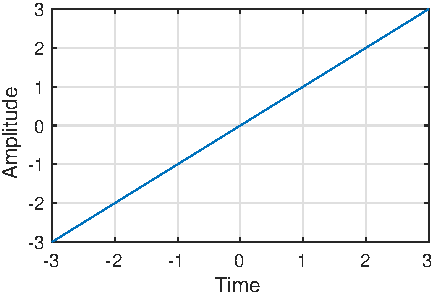
\includegraphics[width=0.5\linewidth]{images/sample-graph.pdf}
		\caption{Sample Diagram}
		\label{fig:universe}
	\end{figure}
\end{verbatim} 
which will produce the output as 
\begin{figure}[!h]
	\centering
	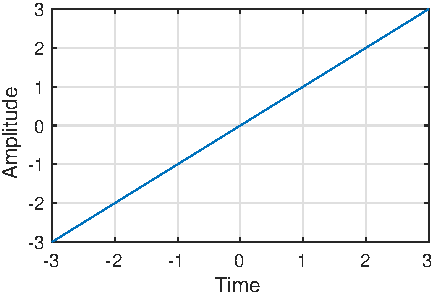
\includegraphics[width=0.5\linewidth]{images/sample-graph.pdf}
	\caption{Sample Diagram}
	\label{fig:universe1}
\end{figure}
\linebreak
More than one figures can be shown adjacent using following code
\begin{verbatim}
	\begin{figure}[h!]
		\centering
		% Left image (a)
		\begin{subfigure}[b]{0.45\linewidth}
			\centering
			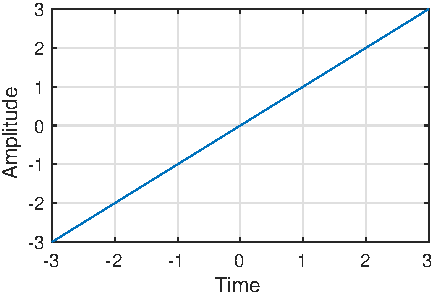
\includegraphics[width=\textwidth]{images/sample-graph.pdf} % replace with your image filename
			\caption{Example Graph}
			\label{fig:fruitsA}
		\end{subfigure}
		\hfill
		% Right image (b)
		\begin{subfigure}[b]{0.45\linewidth}
			\centering
			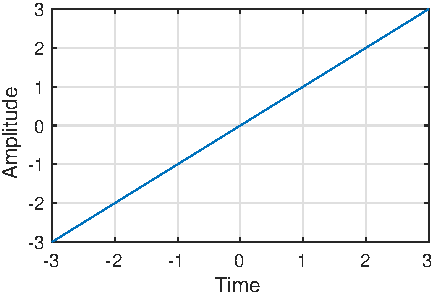
\includegraphics[width=\textwidth]{images/sample-graph.pdf} % replace with your image filename
			\caption{Example Graph}
			\label{fig:fruitsC}
		\end{subfigure}
		
		\caption{Commonly available fruits}
		\label{fig:common_fruits}
	\end{figure}
\end{verbatim}
The above code will produce the results as 
\begin{figure}[h!]
	\centering
	% Left image (a)
	\begin{subfigure}[b]{0.45\linewidth}
		\centering
		\rotatebox{45}{
		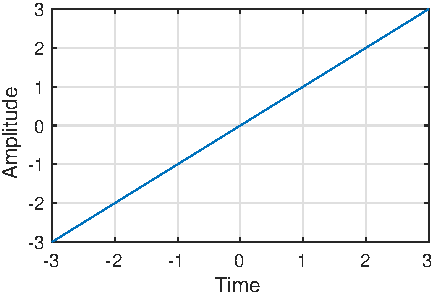
\includegraphics[width=\textwidth]{images/sample-graph.pdf} %	 replace with your image filename
		}
		
	
		\label{fig:fruitsAA}
	\end{subfigure}
	\hfill
	% Right image (b)
	\begin{subfigure}[b]{0.45\linewidth}
		\centering
		\rotatebox{-45}{
		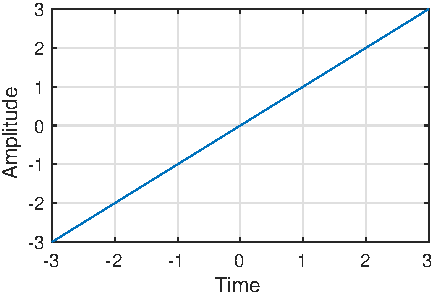
\includegraphics[width=\textwidth]{images/sample-graph.pdf} % replace with your image filename
		}
		\label{fig:fruitsCC}
	\end{subfigure}
	
	\caption{Figures with rotation}
	\label{fig:common_fruitsA}
\end{figure}

\subsection{Pseudo code / Algorithm}
The algorithm or pseudo code can be added using following code
\begin{verbatim}
	\begin{algorithm}
		\caption{An example algorithm with caption}\label{alg:cap}
		\begin{algorithmic}
			\Require $n \geq 0$
			\Ensure $y = x^n$
			\State $y \gets 1$
			\State $X \gets x$
			\State $N \gets n$
			\While{$N \neq 0$}
			\If{$N$ is even}
			\State $X \gets X \times X$
			\State $N \gets \frac{N}{2}$  \Comment{This is a comment}
			\ElsIf{$N$ is odd}
			\State $y \gets y \times X$
			\State $N \gets N - 1$
			\EndIf
			\EndWhile
		\end{algorithmic}
	\end{algorithm}
\end{verbatim}
This code will produce the following output in the report.
\begin{algorithm}
	\caption{An example algorithm with caption}\label{alg:cap}
	\begin{algorithmic}
		\Require $n \geq 0$
		\Ensure $y = x^n$
		\State $y \gets 1$
		\State $X \gets x$
		\State $N \gets n$
		\While{$N \neq 0$}
		\If{$N$ is even}
		\State $X \gets X \times X$
		\State $N \gets \frac{N}{2}$  \Comment{This is a comment}
		\ElsIf{$N$ is odd}
		\State $y \gets y \times X$
		\State $N \gets N - 1$
		\EndIf
		\EndWhile
	\end{algorithmic}
\end{algorithm}
\end{spacing}
	\chapter{System Design}

\section{System Architecture}

This burnout detection system is built using an architecture which comprises several layers including those for collecting data, processing data, performing machine learning tasks, and decision-making.

The system is divided into the following layers: 

\subsection{Data Collection Layer}

This layer is tasked with collecting multi-sourced behavioral data on students. Data is gathered from multiple sources, including academic performance, attendance records, learning management system data, health measures, and social interaction networks.

The data collected is then saved in one main database for further analysis. The issue of data confidentiality is observed by adopting various data anonymization methods.

\subsection{Data Processing Layer}

At this stage, the raw data undergo preprocessing, where missing values are addressed, inconsistencies are resolved, and numerical attributes are scaled. 
Feature extraction and transformation is employed to transform raw behavioral data into structured data that can be used by machine learning algorithms.

\subsection{Feature Engineering Layer}

Provides feature extraction of elements that are important in relation to the processed data. Patterns in the temporal behavior and data are established to create important features, including engagement, stress, and academic performance trends.

It is also possible to create composite features for behavioral patterns like academic stress and social withdrawal.

\subsection{Machine Learning Layer}

The machine learning component is made up of several prediction models that have been trained to identify early symptoms of burnout. Various algorithms like Logistic Regression, Random Forest, Gradient Boosting, and Support Vector Machines are deployed for comparison purposes.

These models are trained using past behavioral information and validated through cross-validation.

\subsection{Prediction and Decision Layer}

This layer calculates the burnout probability score and categorizes the users based on their risk of burnout. Depending on the risk level identified, the system makes valuable suggestions.

The decision layer allows for the early identification of potential burnout cases to prevent an impending crisis.

\subsection{Visualization and Interface Layer}

The last layer displays results in dashboards or reporting systems. Administrators and counselors can view the risks, trends, and alerts in this layer.
This layer enhances user-friendliness and supports evidence-based decision-making.

\textbf{[Insert System Architecture Diagram Here]}


\section{System Workflow}

The process workflow refers to the steps that have to be followed during the burnout identification process. The process begins by collecting raw behavior data from different sources.

Once the data has been collected, it is subjected to pre-processing. During this phase, the inconsistencies in the data are sorted out, and normalization is conducted.

The features obtained from the pre-processed data are further analyzed through feature engineering. This step ensures that the necessary features are extracted. Such features include engagement score, stress levels, and academic trends.

The features obtained from feature engineering are fed into machine learning algorithms to obtain the probability of experiencing burnout.

Finally, the outputs obtained from the process are used to identify different user groups. Each group is assigned actions, which include displaying the results on a visualization screen.

\textbf{[Insert Workflow Diagram Here]}


\section{Data Flow Diagram}





\section{Use Case Diagram}

\begin{figure}
    \centering
    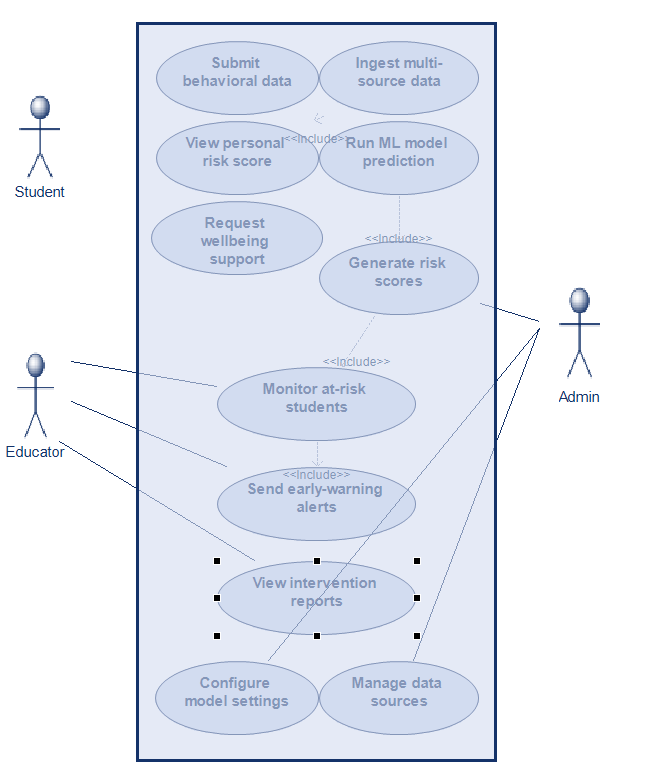
\includegraphics[width=0.7\linewidth]{image.png}
    \caption{use case diagram of burnout signal detection}
    \label{fig:placeholder}
\end{figure}

\section{Class Diagram}




\section{Sequence Diagram}



\textbf{[Insert Sequence Diagram Here]}


\section{Design Considerations}

The system will incorporate the following characteristics:

\begin{itemize}
    \item \textbf{Scalability:} The ability to manage large amounts of data about students and work under institutional settings
    \item \textbf{Accuracy:} High accuracy of predictions through sophisticated machine learning algorithms
    \item \textbf{Security:} The ability to process data securely
    \item \textbf{Modularity:} Distinctiveness between different system components
    \item \textbf{Real-time Processing:} Enables constant monitoring and prediction
\end{itemize}
	\chapter{Methodology and Testing}
\vspace{+10pt}
\section{Methodology}

The suggested system for burnout detection uses an established framework of Machine Learning that looks for detecting early signs of burnout among students with the help of multi-source behavioral data. This method encompasses various stages like data gathering, preprocessing, feature generation, model creation, and risk stratification.

\subsection{Dataset Description and Data Sources}

The database utilized in this experiment has about 16,000 data points based on 1,000 students spanning 16 weeks. Each data point captures behavioral and academic characteristics that reflect the level of student involvement and wellness.

The dataset integrates multiple heterogeneous data sources, including:
\begin{itemize}
    \item Measures for academic success include GPA trends and assignment scores
    \item Attendance patterns and participation rates
    \item Learning Management System activity, which entails logging in and interacting with materials
    \item Library usage that demonstrates study practices
    \item Social engagement measures that denote peer engagement
    \item Wellness measures such as sleep and stress patterns; assignment submission patterns
    \item Assignment submission behavior (on-time, late, or missing)
    \item Help-seeking patterns that may include counseling and academic assistance usage
\end{itemize}

Combining different types of data gives us a clear picture of student behavior, thus allowing us to analyze behavioral patterns, which is critical in identifying signs of stress at the earliest possible time.

\subsection{Data Preprocessing}

Raw data from multiple sources may contain inconsistencies, missing values, and noise. To improve data quality and reliability, the following appropriate preprocessing steps are applied before analysis and model training processes begin.

\begin{itemize}
    \item The mean or median is used for numerical features, whereas the mode is applied for categorical data.
    \item Outliers are detected using IQR analysis and eliminated to avoid biasing model training.
    \item Scaling of the features is done using StandardScaler.
    \item For categorical variables, we use label encoding or one-hot encoding.
\end{itemize}
These steps ensure that the dataset is clean, consistent, and suitable for ML algorithms.

\subsection{Feature Engineering}

Feature extraction is very necessary since burnout is not an observable phenomenon; it is a behavior that can be deduced. Therefore, it is vital to select features that will improve the accuracy of models used for detecting burnout.

The following feature engineering techniques are applied:

\begin{itemize}
    \item \textbf{Temporal Aggregation:} The statistical parameters like mean, standard deviation, minimum, and maximum are calculated over the span of 16 weeks in order to derive behavioral patterns
    \item \textbf{Derived Features:} Parameters like GPA decline parameter, assignment submission percentage, and engagement parameter are derived.
    \item \textbf{Composite Indicators:} Multiple parameters like academic distress parameter and social withdrawal parameter are calculated using relevant parameters.
\end{itemize}
A total of 64 engineered features are generated, which serve as inputs to the predictive models.

\subsection{Model Development}

In order to develop good predictive results, various models of machine learning are employed and analyzed. Different classifiers are used and compared in an effort to select the best classifier for predicting burnout.

\begin{itemize}
    \item Logistic Regression (simple linear baseline model)
    \item Random Forest (ensemble-based model for capturing non-linear relationships)
    \item Gradient Boosting (very efficient boosting method)
    \item Support Vector Machine (classification technique using kernel)
\end{itemize}
These models are chosen to provide a balance between interpretability and predictive power.

\subsection{Training Strategy and Optimization}

The data set is split into training and test datasets in an 80:20 ratio. Stratified five-fold cross validation is used for improving the generalization capacity of the models and avoiding overfitting.

The tuning process for hyperparameters is carried out via grid search and random search methods. Normalization of features is done before training to ensure consistency in scaling.

\subsection{Risk Prediction and Stratification}

The predictions from the trained models give a probability score indicating the possibility of burnout. This is discretized to determine the risk level as follows:

\begin{itemize}
    \item Low Risk (0--40\%)
    \item Medium Risk (40--70\%)
    \item High Risk (70--100\%)
\end{itemize}

This helps the system offer useful information and implement preventive measures for students at risk.
\section{Testing}

\subsection{Testing Strategy}

Evaluation of the system takes place through a combination of hold-out validation and cross-validation techniques.
Validation is done using unseen data to mimic a real-life environment. Comparison of the model performance is carried out using several algorithms.

\subsection{Evaluation Metrics}

For a proper analysis of the performance of the classifier, several metrics can be employed:

\begin{itemize}
    \item \textbf{Accuracy:} This calculates the proportion of accurate predictions made
    \item \textbf{Precision:} This metric checks how accurate are the positive predictions
    \item \textbf{Recall:} The extent to which the algorithm detects burnout
    \item \textbf{F1-Score:} The harmonic mean between the precision and recall values
    \item \textbf{AUC-ROC:} This assesses the model’s ability to distinguish between the two classes
\end{itemize}

Among these, recall and AUC-ROC are given higher importance, as missing a burnout case is more critical than a false positive.

\subsection{Performance Analysis}

Experimental findings show that ensemble models like Random Forest and Gradient Boosting have superior performance compared to basic models because they can detect complex behavior patterns.

The model shows strong prediction power and the capability to identify burnout warning signs around 4-8 weeks before any crucial phase begins.

\subsection{Feature Importance Analysis}

Feature Importance is performed to determine the predictors having the highest impact on burnout. It was found out that

\begin{itemize}
    \item Stress level and sleep quality have significant psychological significance
    \item GPA drop indicates a lack of interest in studies
    \item Assignment submission and class attendance indicate consistency in behavior
\end{itemize}

This analysis also improves interpretability and trust in the model.

\subsection{Validation Using Case Scenarios}

In order to further test the reliability of the system, simulated student records are used. The system can identify risky students due to poor performance, high stress, and lack of engagement.

For such students, the model provides high probability results and suggests possible interventions like counseling and educational assistance.

\subsection{System Reliability and Scalability}

It is able to process large amounts of data, and can be deployed on an organizational level. It has been made with modularity in mind, allowing for better performance and scalability for new demands.

\subsection{Testing Outcome}

The overall testing results confirm that the proposed system:

\begin{itemize}
    \item Precise identification of early signs of burnout 
    \item Offers reliable and meaningful risk categorization 
    \item Facilitates early intervention efforts
    \item Allows for wide-scale implementation among extremely large numbers of students
\end{itemize}
	\include{chapters/chapter6}
	\include{chapters/chapter7} % included 
	\chapter{\MakeUppercase{Conclusion and Further enhancements}} 

The proposed burnout signal detection system demonstrates the effectiveness of a data-driven approach in identifying early indicators of academic burnout. By integrating multiple behavioral data sources such as academic performance, attendance, engagement, and health metrics, the system provides a holistic view of student well-being.

The implementation of machine learning models enables accurate prediction of burnout risk, allowing detection several weeks before critical stages. This early identification supports timely intervention strategies, thereby reducing the likelihood of academic decline and mental health issues.

The system architecture is designed to be modular and scalable, ensuring that it can handle large datasets and adapt to institutional-level deployment. Furthermore, the use of interpretable features and risk classification enhances transparency, making the system practical for real-world use by administrators and counselors.

Overall, the project highlights the potential of combining machine learning and behavioral analytics to address critical challenges in education and student wellness.

\section{Future Work}

Although the proposed system achieves promising results, several enhancements can be explored to further improve its performance and applicability.

\begin{itemize}
    \item Integration of real-time data streams for continuous monitoring and dynamic prediction
    \item Implementation of advanced deep learning models such as LSTM for capturing temporal patterns
    \item Development of a web-based dashboard for real-time visualization and user interaction
    \item Incorporation of additional data sources such as biometric and psychological assessments
    \item Enhancement of model interpretability using explainable AI techniques
    \item Deployment and testing using real-world institutional data while ensuring data privacy compliance
\end{itemize} % included 
	
	%------ Bibliography ----------------------------------------
	\begin{thebibliography}{15}

\bibitem{ref1}
J. Kuzilek, M. Hlosta, and Z. Zdrahal, “Open University Learning Analytics Dataset,” \textit{Scientific Data}, vol. 4, no. 1, 2017.

\bibitem{ref2}
D. Tempelaar, B. Rienties, and Q. Nguyen, “Subjective data, objective data and the role of self-regulation in learning analytics,” \textit{British Journal of Educational Technology}, vol. 46, no. 4, pp. 842–859, 2015.

\bibitem{ref3}
C. Romero and S. Ventura, “Educational data mining: A review of the state of the art,” \textit{IEEE Transactions on Systems, Man, and Cybernetics}, vol. 40, no. 6, pp. 601–618, 2010.

\bibitem{ref4}
S. B. Kotsiantis, C. Pierrakeas, and P. Pintelas, “Predicting students’ performance in distance learning using machine learning techniques,” \textit{Applied Artificial Intelligence}, vol. 18, no. 5, pp. 411–426, 2004.

\bibitem{ref5}
A. Ahmad, N. Ismail, and A. A. Aziz, “The prediction of students’ academic performance using classification data mining techniques,” \textit{Applied Mathematical Sciences}, vol. 9, no. 129, pp. 6415–6426, 2019.

\bibitem{ref6}
G. Dekker, M. Pechenizkiy, and J. Vleeshouwers, “Predicting students dropout: A case study,” in \textit{Proc. International Conference on Educational Data Mining}, 2009.

\bibitem{ref7}
K. E. Arnold and M. D. Pistilli, “Course signals at Purdue: Using learning analytics to increase student success,” in \textit{Proc. Learning Analytics and Knowledge Conference}, 2012.

\bibitem{ref8}
R. S. J. d. Baker and R. Inventado, “Educational data mining and learning analytics,” in \textit{Learning Analytics}, Springer, 2014, pp. 61–75.

\bibitem{ref9}
C. Maslach and M. P. Leiter, “Understanding the burnout experience: Recent research and its implications,” \textit{World Psychiatry}, vol. 15, no. 2, pp. 103–111, 2016.

\bibitem{ref10}
H. Schaufeli, W. B. Schaufeli, and D. Enzmann, “The burnout companion to study and practice: A critical analysis,” \textit{Taylor \& Francis}, 1998.

\bibitem{ref11}
T. Mikolov et al., “Efficient estimation of word representations in vector space,” \textit{arXiv preprint arXiv:1301.3781}, 2013.

\bibitem{ref12}
F. Pedregosa et al., “Scikit-learn: Machine learning in Python,” \textit{Journal of Machine Learning Research}, vol. 12, pp. 2825–2830, 2011.

\bibitem{ref13}
L. Breiman, “Random forests,” \textit{Machine Learning}, vol. 45, no. 1, pp. 5–32, 2001.

\bibitem{ref14}
J. Friedman, “Greedy function approximation: A gradient boosting machine,” \textit{Annals of Statistics}, vol. 29, no. 5, pp. 1189–1232, 2001.

\bibitem{ref15}
C. Cortes and V. Vapnik, “Support-vector networks,” \textit{Machine Learning}, vol. 20, no. 3, pp. 273–297, 1995.

\bibitem{ref16}
S. Jayaprakash, E. Moody, E. J. Lauría, J. R. Regan, and J. D. Baron, “Early alert of academically at-risk students: An open source analytics initiative,” \textit{Journal of Learning Analytics}, vol. 1, no. 1, pp. 6–47, 2014.

\bibitem{ref17}
M. S. Hussain, W. Zhu, W. Zhang, and S. M. Abidi, “Student engagement predictions in an e-learning system and their impact on student course assessment scores,” \textit{Computational Intelligence and Neuroscience}, 2018.

\bibitem{ref18}
A. S. Alharthi, “Student engagement and learning outcomes in higher education: A review,” \textit{International Journal of Educational Technology}, vol. 5, no. 2, pp. 45–52, 2019.

\bibitem{ref19}
E. T. Bradlow, D. Hutchinson, and P. S. Fader, “Behavioral analytics in education: Applications and challenges,” \textit{Journal of Educational Data Science}, vol. 3, no. 1, pp. 1–15, 2020.

\bibitem{ref20}
J. P. Campbell, P. B. DeBlois, and D. G. Oblinger, “Academic analytics: A new tool for a new era,” \textit{EDUCAUSE Review}, vol. 42, no. 4, pp. 40–57, 2007.

\end{thebibliography} 
	%------ Appendices ----------------------------------------
	\newpage
	\include{appendix/sourcecode}	% comment if not necessary
	\newpage
	\include{appendix/publication}	% comment if not necessary
	
\end{document}